\documentclass{article}
\usepackage{amssymb,amsmath}
\usepackage{ifxetex,ifluatex}
\ifxetex
  \usepackage{fontspec,xltxtra,xunicode}
  \defaultfontfeatures{Mapping=tex-text,Scale=MatchLowercase}
\else
  \ifluatex
    \usepackage{fontspec}
    \defaultfontfeatures{Mapping=tex-text,Scale=MatchLowercase}
  \else
    \usepackage[utf8]{inputenc}
  \fi
\fi
\usepackage{ctable}
\usepackage{float} % provides the H option for float placement
\usepackage{graphicx}
% We will generate all images so they have a width \maxwidth. This means
% that they will get their normal width if they fit onto the page, but
% are scaled down if they would overflow the margins.
\makeatletter
\def\maxwidth{\ifdim\Gin@nat@width>\linewidth\linewidth
\else\Gin@nat@width\fi}
\makeatother
\let\Oldincludegraphics\includegraphics
\renewcommand{\includegraphics}[1]{\Oldincludegraphics[width=\maxwidth]{#1}}
\ifxetex
  \usepackage[setpagesize=false, % page size defined by xetex
              unicode=false, % unicode breaks when used with xetex
              xetex]{hyperref}
\else
  \usepackage[unicode=true]{hyperref}
\fi
\hypersetup{breaklinks=true, pdfborder={0 0 0}}
\setlength{\parindent}{0pt}
\setlength{\parskip}{6pt plus 2pt minus 1pt}
\setlength{\emergencystretch}{3em}  % prevent overfull lines
\setcounter{secnumdepth}{0}

\title{Crosstable}
\author{Rapport package team @ https://github.com/aL3xa/rapport}
\date{2011--04--26 20:25 CET}

\begin{document}
\maketitle

\subsection{Description}

Returning the Chi-squared test of two given variables with count,
percentages and Pearson's residuals table.

\subsubsection{Variable description}

Two variables specified:

\begin{itemize}
\item
  ``gender'' (``Gender'') with 709 and
\item
  ``dwell'' (``Dwelling'') with 709 valid values.
\end{itemize}
\subsubsection{Counts}

\ctable[pos = H, center, botcap]{llll}
{% notes
}
{% rows
\FL
 & \textbf{city} & \textbf{small town} & \textbf{village}
\ML
male & 380 & 30 & 22
\\\noalign{\medskip}
female & 262 & 6 & 9
\LL
}

\subsubsection{Percentages}

\ctable[pos = H, center, botcap]{llll}
{% notes
}
{% rows
\FL
 & \textbf{city} & \textbf{small town} & \textbf{village}
\ML
male & 0.5360 & 0.0423 & 0.0310
\\\noalign{\medskip}
female & 0.3695 & 0.0085 & 0.0127
\LL
}

\paragraph{Row percentages}

\ctable[pos = H, center, botcap]{llll}
{% notes
}
{% rows
\FL
 & \textbf{city} & \textbf{small town} & \textbf{village}
\ML
male & 0.8796 & 0.0694 & 0.0509
\\\noalign{\medskip}
female & 0.9458 & 0.0217 & 0.0325
\LL
}

\paragraph{Column percentages}

\ctable[pos = H, center, botcap]{llll}
{% notes
}
{% rows
\FL
 & \textbf{city} & \textbf{small town} & \textbf{village}
\ML
male & 0.5919 & 0.8333 & 0.7097
\\\noalign{\medskip}
female & 0.4081 & 0.1667 & 0.2903
\LL
}

\subsubsection{Chi-squared test}

\ctable[pos = H, center, botcap]{llll}
{% notes
}
{% rows
\FL
 & \textbf{X-squared} & \textbf{df} & \textbf{p-value}
\ML
X-squared & 9.72 & 2.00 & 0.01
\LL
}

It seems that a real association can be pointed out between
\emph{gender} and \emph{dwell} by the \emph{Pearson's Chi-squared test}
(χ=9.7188 at the degree of freedom being 2) at the significance level of
0.0078. Based on Goodman and Kruskal's lambda it seems that \emph{dwell}
(λ=0.7581) has an effect on \emph{gender} (λ=0) if we assume both
variables to be nominal. The association between the two variables seems
to be weak based on Cramer's V (0.0828).

\paragraph{Pearson's residuals}

\ctable[pos = H, center, botcap]{llll}
{% notes
}
{% rows
\FL
 & \textbf{city} & \textbf{small town} & \textbf{village}
\ML
male & --2.9409 & 2.8277 & 1.1713
\\\noalign{\medskip}
female & 2.9409 & --2.8277 & --1.1713
\LL
}

\paragraph{Mosaic chart}

\begin{figure}[htbp]
\centering
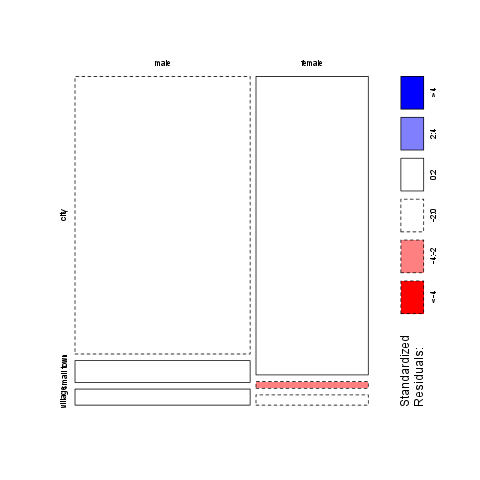
\includegraphics{66ba5aa603e08fec150848bb688f0953.png}
\caption{}
\end{figure}

\subsection{Description}

Returning the Chi-squared test of two given variables with count,
percentages and Pearson's residuals table.

\subsubsection{Variable description}

Two variables specified:

\begin{itemize}
\item
  ``email'' (``Email usage'') with 709 and
\item
  ``dwell'' (``Dwelling'') with 709 valid values.
\end{itemize}
\subsubsection{Counts}

\ctable[pos = H, center, botcap]{llll}
{% notes
}
{% rows
\FL
 & \textbf{city} & \textbf{small town} & \textbf{village}
\ML
never & 12 & 0 & 1
\\\noalign{\medskip}
very rarely & 34 & 1 & 3
\\\noalign{\medskip}
rarely & 46 & 3 & 2
\\\noalign{\medskip}
sometimes & 76 & 6 & 8
\\\noalign{\medskip}
often & 113 & 11 & 5
\\\noalign{\medskip}
very often & 106 & 5 & 5
\\\noalign{\medskip}
always & 255 & 10 & 7
\LL
}

\subsubsection{Percentages}

\ctable[pos = H, center, botcap]{llll}
{% notes
}
{% rows
\FL
 & \textbf{city} & \textbf{small town} & \textbf{village}
\ML
never & 0.0169 & 0.0000 & 0.0014
\\\noalign{\medskip}
very rarely & 0.0480 & 0.0014 & 0.0042
\\\noalign{\medskip}
rarely & 0.0649 & 0.0042 & 0.0028
\\\noalign{\medskip}
sometimes & 0.1072 & 0.0085 & 0.0113
\\\noalign{\medskip}
often & 0.1594 & 0.0155 & 0.0071
\\\noalign{\medskip}
very often & 0.1495 & 0.0071 & 0.0071
\\\noalign{\medskip}
always & 0.3597 & 0.0141 & 0.0099
\LL
}

\paragraph{Row percentages}

\ctable[pos = H, center, botcap]{llll}
{% notes
}
{% rows
\FL
 & \textbf{city} & \textbf{small town} & \textbf{village}
\ML
never & 0.9231 & 0.0000 & 0.0769
\\\noalign{\medskip}
very rarely & 0.8947 & 0.0263 & 0.0789
\\\noalign{\medskip}
rarely & 0.9020 & 0.0588 & 0.0392
\\\noalign{\medskip}
sometimes & 0.8444 & 0.0667 & 0.0889
\\\noalign{\medskip}
often & 0.8760 & 0.0853 & 0.0388
\\\noalign{\medskip}
very often & 0.9138 & 0.0431 & 0.0431
\\\noalign{\medskip}
always & 0.9375 & 0.0368 & 0.0257
\LL
}

\paragraph{Column percentages}

\ctable[pos = H, center, botcap]{llll}
{% notes
}
{% rows
\FL
 & \textbf{city} & \textbf{small town} & \textbf{village}
\ML
never & 0.0187 & 0.0000 & 0.0323
\\\noalign{\medskip}
very rarely & 0.0530 & 0.0278 & 0.0968
\\\noalign{\medskip}
rarely & 0.0717 & 0.0833 & 0.0645
\\\noalign{\medskip}
sometimes & 0.1184 & 0.1667 & 0.2581
\\\noalign{\medskip}
often & 0.1760 & 0.3056 & 0.1613
\\\noalign{\medskip}
very often & 0.1651 & 0.1389 & 0.1613
\\\noalign{\medskip}
always & 0.3972 & 0.2778 & 0.2258
\LL
}

\subsubsection{Chi-squared test}

\ctable[pos = H, center, botcap]{llll}
{% notes
}
{% rows
\FL
 & \textbf{X-squared} & \textbf{df} & \textbf{p-value}
\ML
X-squared & 14.37 & 12.00 & 0.28
\LL
}

It seems that no real association can be pointed out between
\emph{email} and \emph{dwell} by the \emph{Pearson's Chi-squared test}
(χ=14.366 at the degree of freedom being 12) at the significance level
of 0.2779. For this end no other statistical tests were performed.

\paragraph{Pearson's residuals}

\ctable[pos = H, center, botcap]{llll}
{% notes
}
{% rows
\FL
 & \textbf{city} & \textbf{small town} & \textbf{village}
\ML
never & 0.2187 & --0.8417 & 0.5908
\\\noalign{\medskip}
very rarely & --0.2332 & --0.7060 & 1.0915
\\\noalign{\medskip}
rarely & --0.0897 & 0.2717 & --0.1634
\\\noalign{\medskip}
sometimes & --2.1192 & 0.7349 & 2.2426
\\\noalign{\medskip}
often & --1.2678 & 1.9731 & --0.3048
\\\noalign{\medskip}
very often & 0.3338 & --0.4116 & --0.0357
\\\noalign{\medskip}
always & 2.2980 & --1.3407 & --1.8480
\LL
}

\paragraph{Mosaic chart}

\begin{figure}[htbp]
\centering
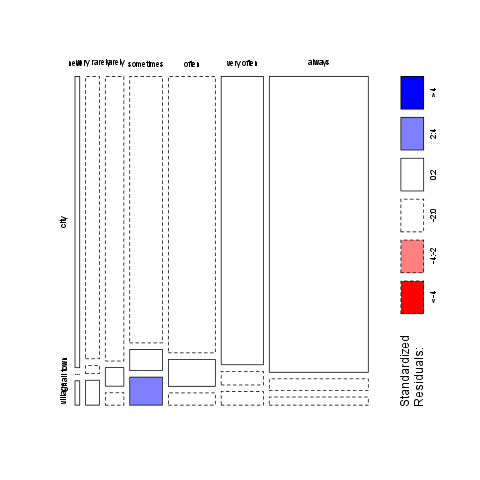
\includegraphics{b26fc463113e2f16bc930c620677e929.png}
\caption{}
\end{figure}

\end{document}
